[19 v\textsuperscript{o}] et parallelos\protect\index{Sachverzeichnis}{circulus parallelus}. Est enim angulus ad meridianos\protect\index{Sachverzeichnis}{meridianus} complementum anguli ad parallelos\protect\index{Sachverzeichnis}{circulus parallelus}.\pend \pstart Deprehendere flexum navis\protect\index{Sachverzeichnis}{navis}, \edtext{navi}{\lemma{navis,}\Afootnote{ \textit{ (1) }\ alligetur \textit{ (2) }\ navi \textit{ L}}} grandi \edtext{addatur exigua puncto aquae insistens,}{\lemma{grandi}\Afootnote{ \textit{ (1) }\ exigua \textit{(a)}\ rotunda seu conica in puncto insistens aquae \textit{(b)}\ u vel v navi\protect\index{Sachverzeichnis}{navis|textit} grandi parallela \textit{ (2) }\ addatur exigua puncto aquae insistens, \textit{ L}}} nec proinde mobilis, nisi circa unum axem, haec suam lineam cursus seu proram et puppim semper parallelam seu coincidentem teneat lineae majoris. Flexus ejus dabunt exacte flexus majoris. Non enim flectetur nisi in uno puncto. Sola quaestio est quomodo efficiatur, ut persequatur majorem, hoc fiet, vel si ante eam agatur vel ei alligetur, ita enim nave\protect\index{Sachverzeichnis}{navis} se flectente cum ea non flectetur, nisi ab homine dioptram ubi hoc sentit adhibente.\pend
   \vspace{5mm}
   \begin{center}
   %\begin{wrapfigure}{l}{0.6\textwidth}          
   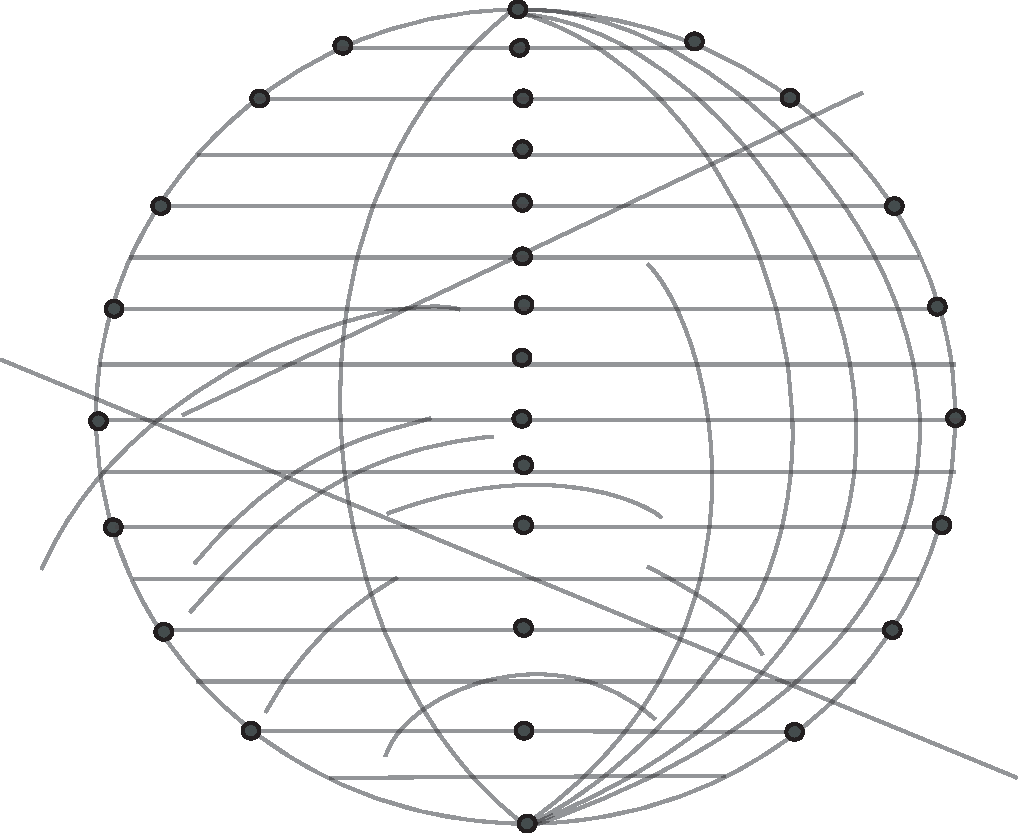
\includegraphics[width=0.8\textwidth]{images/38_19v}\\
   %\caption{Bildbeschreibung}
   \textit{[Fig. 1, tlw. Blindzeichnung]}\\
   \end{center}